\documentclass[12pt, a4paper, oneside, UTF8]{ctexart}
\usepackage{amsmath, amsthm, amssymb, bm, color, framed, graphicx, hyperref, mathrsfs}
\usepackage{geometry}
\usepackage{caption}
\geometry{left = 2.5 cm, right = 2.5 cm, top = 2.5 cm, bottom = 2.5 cm}

\title{\textbf{作业13}\\{\small (数值算法与案例分析)}}
\author{李维杰}
\date{\today}
\linespread{1.5}
\definecolor{shadecolor}{RGB}{241, 241, 255}
\newcounter{problemname}
\newenvironment{problem}{\begin{shaded}\stepcounter{problemname}\par\noindent\textbf{题目\arabic{problemname}. }}{\end{shaded}\par}
\newenvironment{solution}{\par\noindent\textbf{解答. }}{\par}
\newenvironment{note}{\par\noindent\textbf{注记. }}{\par}

\newcommand{\pll}{\kern 0.56em/\kern -0.8em /\kern 0.56em}

\begin{document}

\maketitle

\begin{problem}
    给定对称正定阵$A \in \mathbb{R}^{n \times n}$和向量$b \in \mathbb{R}^{n}$. 假设$\mathcal{V}$是$\mathbb{R}^{n}$的一个子空间.证明:
    $$x_0 = \arg{\min_{x\in\mathcal{V}}{{\left\lVert{x - A^{-1}b}\right\rVert}_{A}}}$$成立当且仅当$b - Ax_0 \in \mathcal{V}^{\bot}$(正交补由标准内积定义).
\end{problem}

\begin{solution}
    设$A^{-1} b = x_* + x_{\bot}$, 其中$x_* \in \mathcal{V}$, $x_{\bot} \in \mathcal{V}^{\bot}$, 则$x_0 = x_*$. 这等价于$$b - Ax_0 = Ax_{\bot} \in \mathcal{V}^{\bot}.$$
\end{solution}

\begin{problem}
    给定列满秩矩阵$A \in \mathbb{R}^{m \times n}$和向量$b \in \mathbb{R}^{m}$.通过解最小二乘问题$\min_{x}{{\left\lVert{Ax - b}\right\rVert}_{2}}$, CG算法可以被用于解决正规方程$A^T Ax = A^T b$.
    请为该方法提供详细的迭代方案. 并确保避免使用操作$v \rightarrow A^T Av$.
\end{problem}

\begin{solution}
    做$n$步迭代.对于第$k$步迭代,依次进行以下操作
    \begin{align*}
        \left\{
            \begin{array}{ll}
                r_{k} = r_{k-1} - {\alpha}_{k-1} A p_{k-1} \\
                {\beta}_{k-1} = \frac{p_{k-1}^* A r_k}{p_{k-1}^* A p_{k-1}} \\
                p_{k} = r_{k} - {\beta}_{k-1} p_{k-1} \\
                {\alpha}_{k} = \frac{r_k^* p_k}{p_k^* A p_k} \\
                x_{k+1} = x_k + {\alpha}_{k} p_k
            \end{array}
        \right. ,
    \end{align*}
    其中初始化$p_0 = r_0 = b, x_0 = 0, {\alpha}_0 = \frac{r_0^* p_0}{p_0^* A p_0}, x_1 = p_0 {\alpha}_0.$
\end{solution}

\begin{problem}
    使用CG算法解单位正方形$[0,1]^2$上的2D拉普拉斯方程$$\frac{\partial^2 u}{\partial x^2} + \frac{\partial^2 u}{\partial y^2} = 0.$$
    该方程有边界条件$$u(0,y)=u(1,y)=u(x,1)=0,y(x,0)=\sin(\pi x).$$
    可视化解和收敛历程.
\end{problem}

\begin{solution}
    (代码见Problem3.m)
    \begin{figure}[h]
        \centering
        \begin{minipage}[b]{0.3\textwidth}
            \centering
            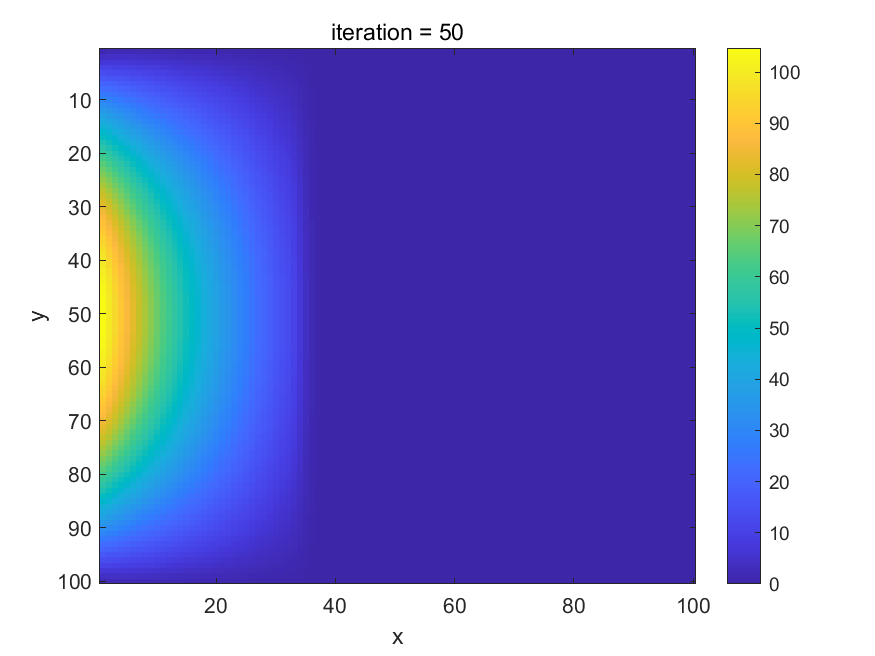
\includegraphics[width=\textwidth]{Problem3_1.png}
            \caption{iter=50}
        \end{minipage}
        \begin{minipage}[b]{0.3\textwidth}
            \centering
            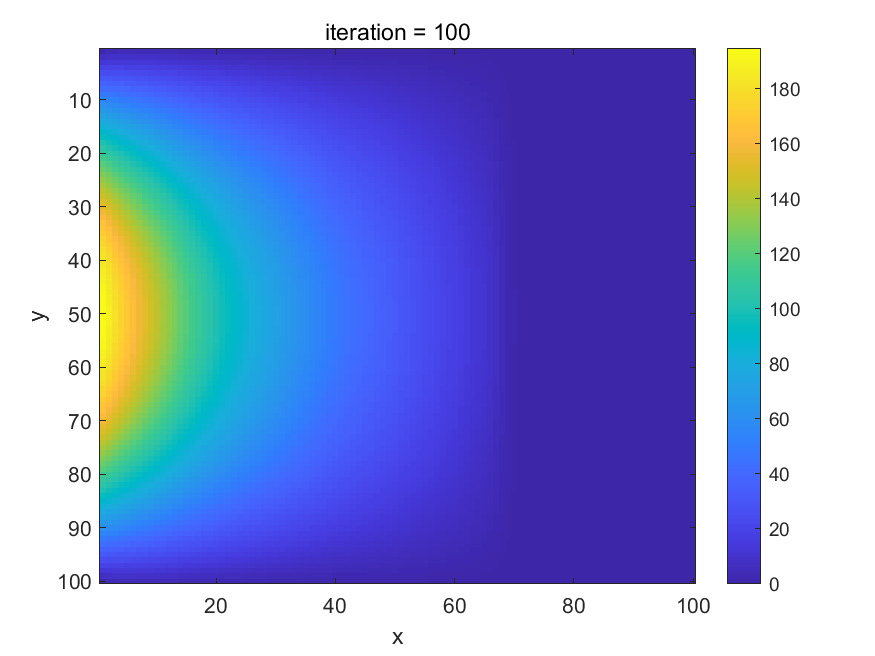
\includegraphics[width=\textwidth]{Problem3_2.png}
            \caption{iter=100}
        \end{minipage}
        \begin{minipage}[b]{0.3\textwidth}
            \centering
            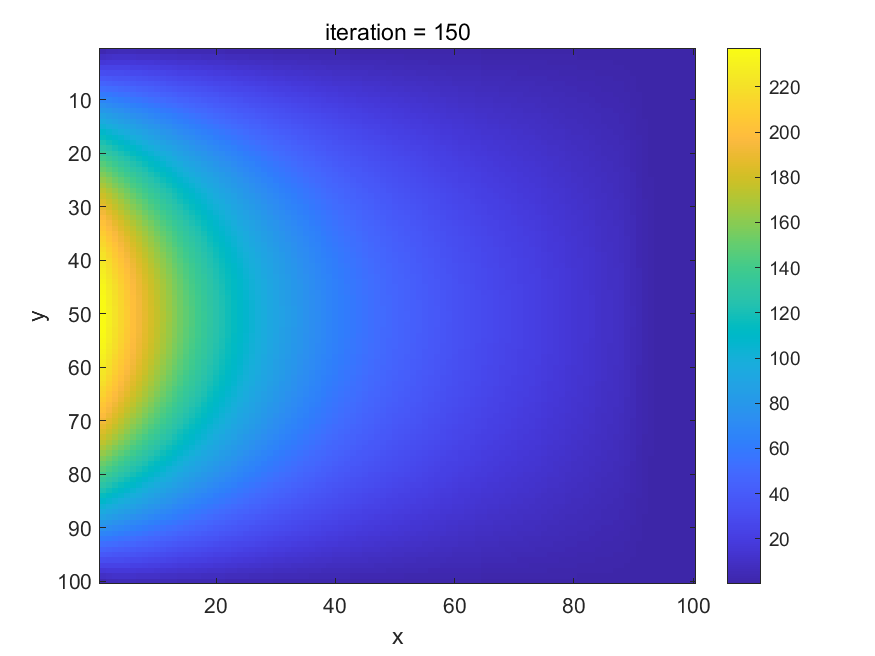
\includegraphics[width=\textwidth]{Problem3_3.png}
            \caption{iter=150}
        \end{minipage}
    \end{figure}
    \begin{figure}[h]
        \centering
        \begin{minipage}[b]{0.3\textwidth}
            \centering
            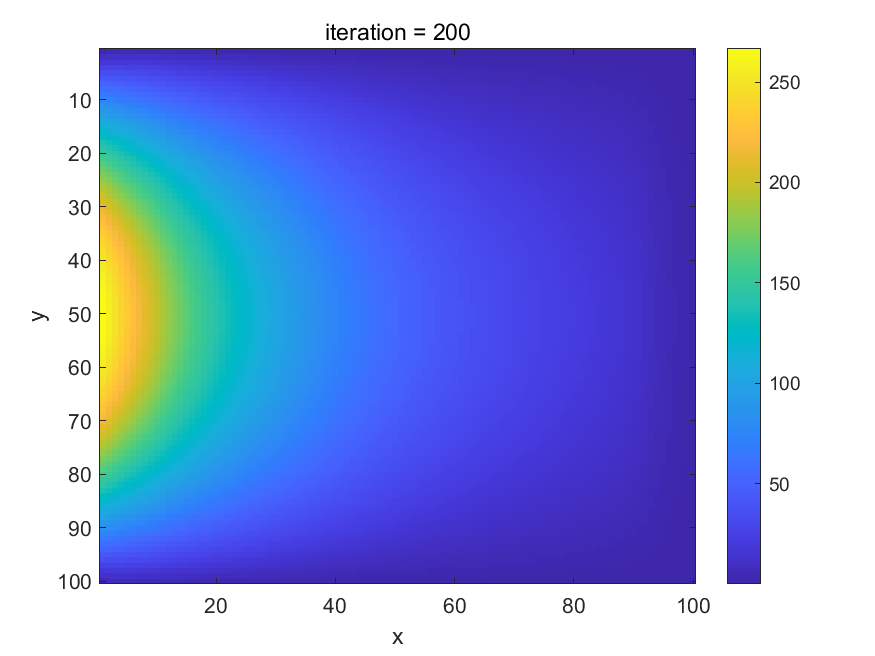
\includegraphics[width=\textwidth]{Problem3_4.png}
            \caption{iter=200}
        \end{minipage}
        \begin{minipage}[b]{0.3\textwidth}
            \centering
            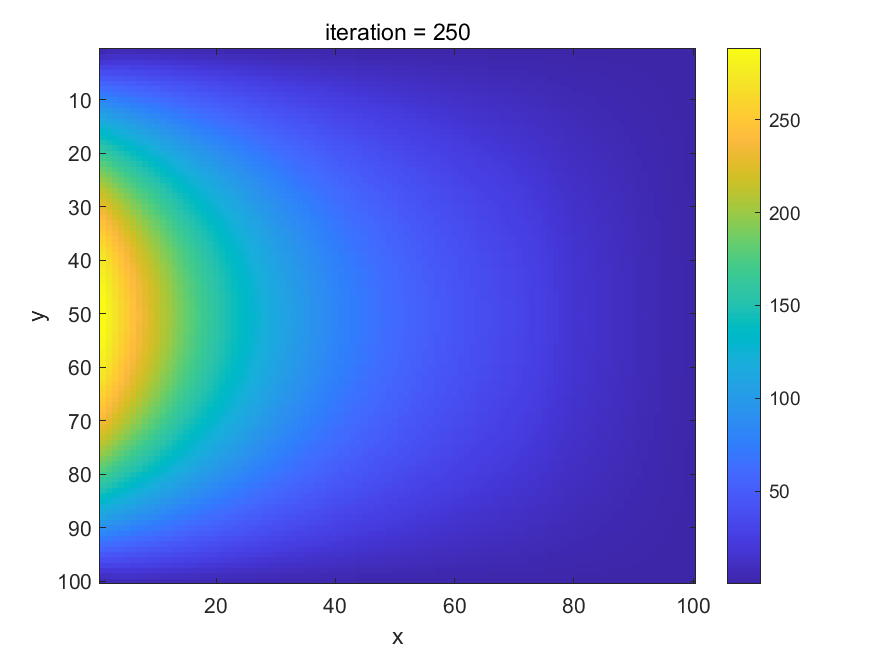
\includegraphics[width=\textwidth]{Problem3_5.png}
            \caption{iter=250}
        \end{minipage}
        \begin{minipage}[b]{0.3\textwidth}
            \centering
            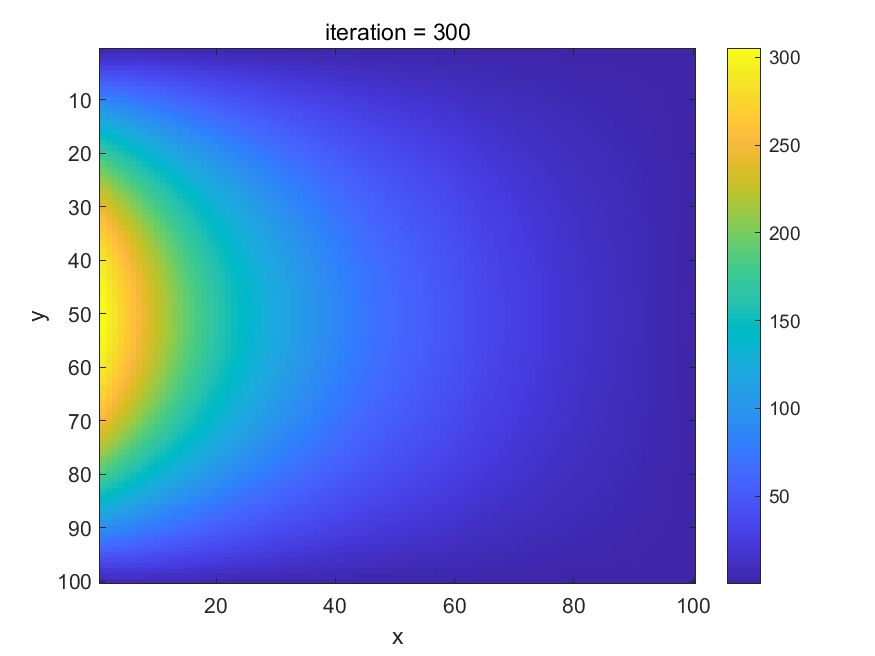
\includegraphics[width=\textwidth]{Problem3_6.png}
            \caption{iter=300}
        \end{minipage}
        \captionsetup{labelformat=empty}  % 禁用编号
        \caption{CG算法(初始设定$u=0$)}  % 只显示标题,没有编号
    \end{figure}
    \begin{figure}[htbp]
        \centering
        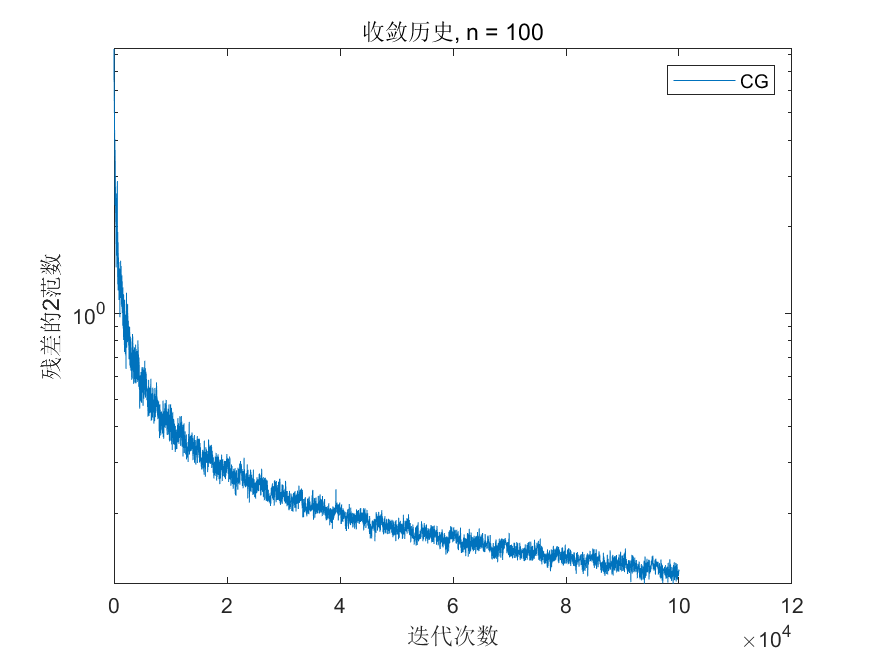
\includegraphics[scale=0.8]{Convergence_History.png}
        \captionsetup{labelformat=empty}
        \caption{CG算法的收敛历程}
    \end{figure}
\end{solution}
\newpage
\begin{problem}
    针对对称特征值问题使用Lanczos算法, 并用一些稀疏Hermite阵测试它. 说明Ritz对的收敛性和Lanczos向量的正交性.
\end{problem}

\begin{solution}
    (代码见Problem4.m)
    \begin{figure}[h]
        \centering
        \begin{minipage}[b]{0.45\textwidth}
            \centering
            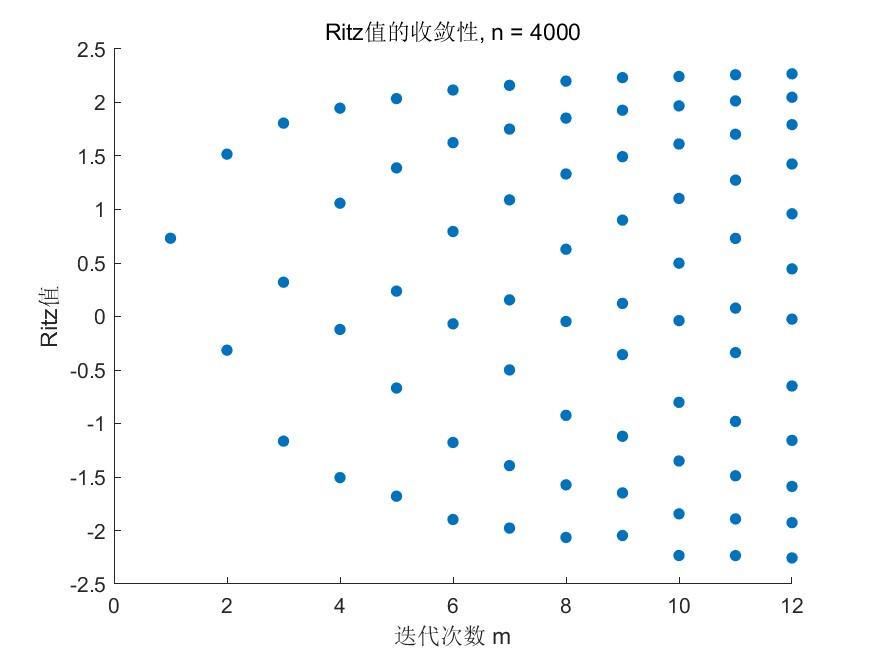
\includegraphics[width=\textwidth]{Problem4_Ritz.jpg}
            \caption{Ritz值的收敛性}
        \end{minipage}
        \begin{minipage}[b]{0.45\textwidth}
            \centering
            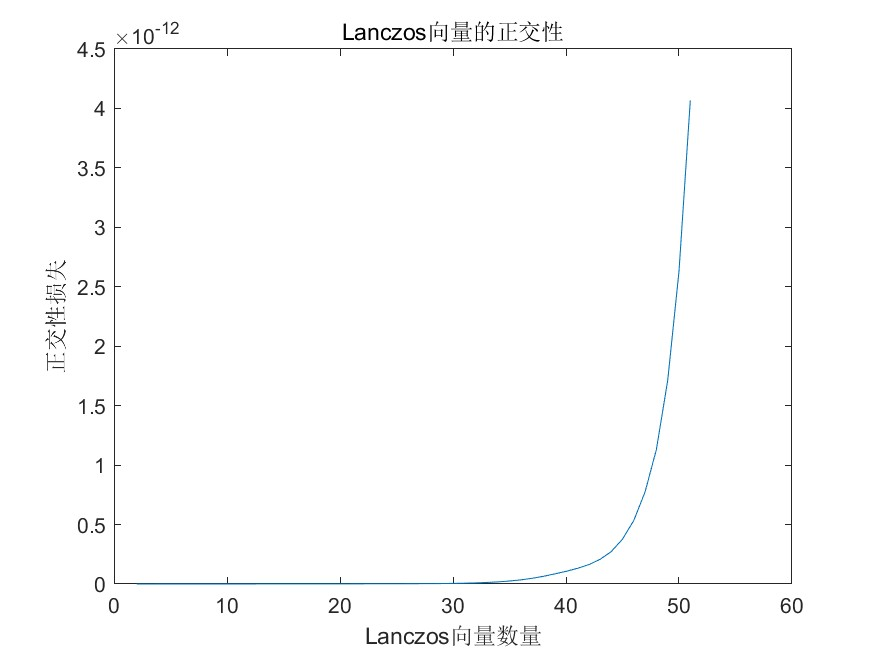
\includegraphics[width=\textwidth]{Problem4_Ortho.jpg}
            \caption{Lanczos向量的正交性}
        \end{minipage}
    \end{figure}
\end{solution}
\end{document}